\documentclass[a4paper,12pt]{article}

\usepackage[utf8]{inputenc}
\usepackage[spanish]{babel}
\usepackage{amsmath, amssymb}
\usepackage{graphicx}
\usepackage{float}
\usepackage{booktabs}
\usepackage{xcolor}
\usepackage{listings}
\usepackage{caption}
\usepackage{fancyhdr}
\usepackage{hyperref}
\usepackage{tikz}
\usepackage{tabularx}

\hypersetup{
    colorlinks=true,
    linkcolor=blue,
    urlcolor=blue,
    pdftitle={Práctica 5 - Comunicacion UART},
}

% === Definición de colores similares a Vivado ===
\definecolor{vivadoKeyword}{rgb}{0.6,0.0,0.6}
\definecolor{vivadoComment}{rgb}{0.0,0.5,0.0}
\definecolor{vivadoString}{rgb}{0.5,0.2,0.0}
\definecolor{vivadoBackground}{rgb}{0.97,0.97,0.97}

\lstdefinelanguage{VHDL}{
    morekeywords={library, use, entity, is, port, in, out, end, architecture, of, begin, signal, if, then, else, when, others, xor, and, or, not},
    sensitive=true,
    morecomment=[l]--,
    morestring=[b]",
}

\lstset{
    language=VHDL,
    backgroundcolor=\color{vivadoBackground},
    keywordstyle=\color{vivadoKeyword}\bfseries,
    commentstyle=\color{vivadoComment}\itshape,
    stringstyle=\color{vivadoString},
    basicstyle=\ttfamily\small,
    numbers=left,
    numberstyle=\tiny,
    numbersep=5pt,
    frame=single,
    breaklines=true,
    tabsize=2,
    captionpos=b
}

\title{Práctica N°5: Comunicación UART}
\date{}

\begin{document}
\maketitle
\tableofcontents
\newpage

\section{Objetivos}

\subsection{Objetivo General}
Establecer la comunicación UART entre el ordenador y la tarjeta Nexys A7-100T, permitiendo la transmisión y recepción de caracteres a través de un software de terminal (como PuTTY), y comprendiendo de manera práctica el funcionamiento de este protocolo de comunicación serie.

\subsection{Objetivos Específicos}
\begin{itemize}
    \item Configurar la interfaz UART en la tarjeta Nexys para recibir y enviar datos.
    \item Utilizar un software de terminal (PuTTY) para establecer conexión con la tarjeta, enviar caracteres y observar las respuestas.
    \item Implementar la lógica en VHDL para que la tarjeta:
    \begin{itemize}
        \item Reenvíe (echo) los caracteres numéricos recibidos.
        \item Genere el mensaje \texttt{'error'} cuando se reciban caracteres no numéricos.
    \end{itemize}
    \item Comprender el flujo completo de comunicación UART desde la configuración del hardware hasta la interacción con el software en el ordenador.
    \item Promover el uso de herramientas de simulación y prueba que faciliten la depuración y comprensión del sistema.
\end{itemize}

\section{Marco Teórico}

\subsection{Comunicación UART}
La comunicación \textbf{UART} (Universal Asynchronous Receiver/Transmitter) es un protocolo de transmisión serie asíncrono ampliamente utilizado para el intercambio de datos entre dispositivos electrónicos. Su característica principal es que no requiere un reloj compartido entre emisor y receptor, ya que ambos extremos deben estar configurados con la misma velocidad de transmisión (\textit{baud rate}).

En este protocolo los datos se transmiten bit a bit a través de una línea, siguiendo un formato estándar:
\begin{itemize}
    \item \textbf{Bit de inicio (Start bit):} indica al receptor que comienza la transmisión.
    \item \textbf{Bits de datos:} normalmente 7 u 8 bits, que representan la información a transmitir.
    \item \textbf{Bit de paridad (opcional):} se utiliza para la detección de errores simples.
    \item \textbf{Bits de parada (Stop bits):} uno o dos bits que señalan el final de la transmisión.
\end{itemize}

En la Figura~\ref{fig:uart-frame} se muestra el formato de una trama UART típica.

\begin{figure}[H]
    \centering
    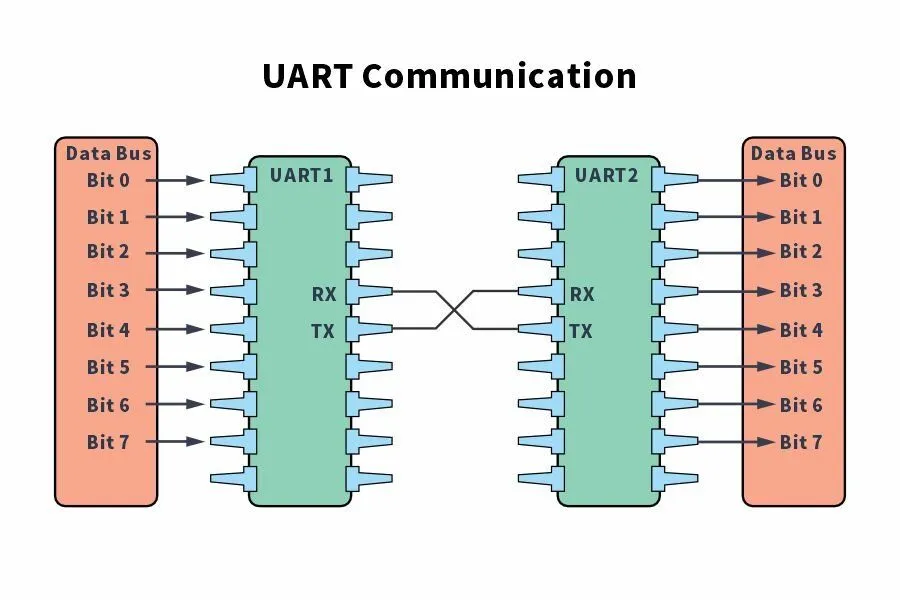
\includegraphics[width=0.7\textwidth]{uart.png}
    \caption{Estructura básica de una trama UART.}
    \label{fig:uart-frame}
\end{figure}

\subsection{Parámetros de configuración}
Para que la comunicación UART funcione correctamente, tanto el ordenador como la tarjeta Nexys deben compartir los mismos parámetros:
\begin{itemize}
    \item \textbf{Velocidad de transmisión (baud rate):} número de bits enviados por segundo (ejemplo: 115200 bps).
    \item \textbf{Bits de datos:} cantidad de bits que representan cada carácter (8 bits en la mayoría de los casos).
    \item \textbf{Paridad:} puede ser \texttt{None}, \texttt{Even} o \texttt{Odd}. En esta práctica no se usará paridad.
    \item \textbf{Bits de parada:} normalmente se usa un bit de parada.
\end{itemize}

\subsection{Uso de PuTTY para la comunicación}
\textbf{PuTTY} es un software de terminal que permite establecer comunicación serie con la tarjeta Nexys mediante el puerto COM del ordenador. Su uso facilita la prueba e interacción con el diseño implementado en VHDL.

Los pasos principales para su configuración son los siguientes:
\begin{enumerate}
    \item Instalar PuTTY en el ordenador (descarga gratuita desde \url{https://www.putty.org/}).
    \item Conectar la tarjeta Nexys al PC mediante el cable USB.
    \item Identificar el puerto COM asignado a la tarjeta en el administrador de dispositivos.
    \item Abrir PuTTY y seleccionar la opción \textbf{Serial} en la pantalla inicial.
    \item Configurar el puerto COM detectado, la velocidad (9600), 8 bits de datos, sin paridad, y 1 bit de parada (formato 8N1).
\end{enumerate}

En las siguientes Figuras se muestra la ventana de configuración de PuTTY con los parámetros requeridos.

\begin{figure}[H]
    \centering
    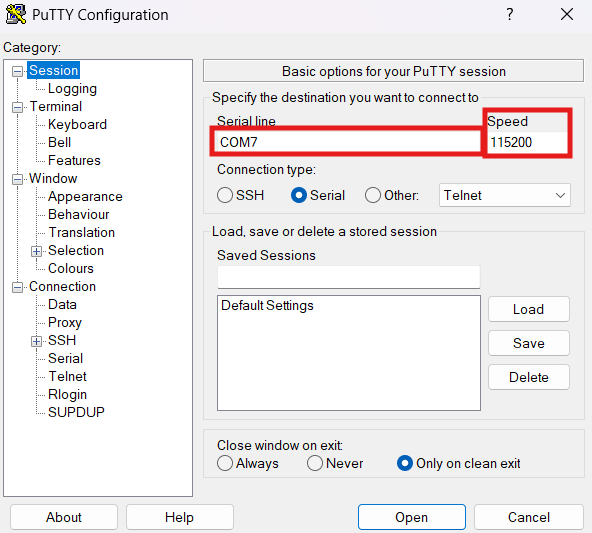
\includegraphics[width=0.6\textwidth]{Putty/com.png}
    \caption{Configuración de PuTTY para la práctica de comunicación UART referente al puerto COM y baud rate.}
    \label{fig:putty-config}
\end{figure}

\begin{figure}[H]
    \centering
    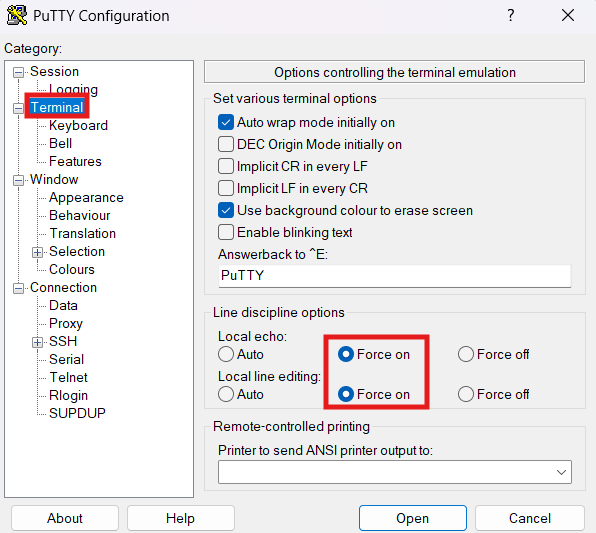
\includegraphics[width=0.6\textwidth]{Putty/terminal.png}
    \caption{Configuración de PuTTY para la práctica de comunicación UART referente a la habilitación de envió.}
    \label{fig:putty-config}
\end{figure}

\begin{figure}[H]
    \centering
    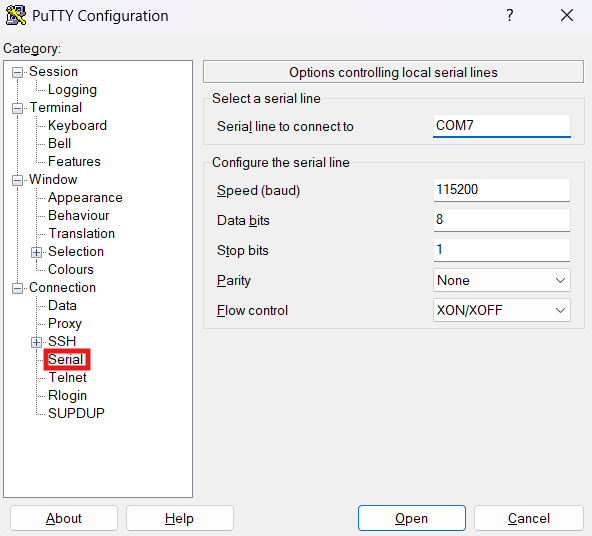
\includegraphics[width=0.6\textwidth]{Putty/serial.png}
    \caption{Configuración de PuTTY para la práctica de comunicación UART referente al serial.}
    \label{fig:putty-config}
\end{figure}

\section{Descripción del Código}

\subsection{Módulo \texttt{UART\_RX}}

El módulo \texttt{uart\_rx} implementa el receptor UART. Su función es detectar los bits que llegan por la línea serie \texttt{rx}, reconstruir el byte transmitido y notificar mediante la señal \texttt{rx\_done} cuando un dato válido ha sido recibido.

\begin{lstlisting}[language=VHDL, caption={Código completo del módulo UART\_RX}, label={lst:uart_rx}]
library IEEE;
use IEEE.STD_LOGIC_1164.ALL;
use IEEE.NUMERIC_STD.ALL;

entity uart_rx is
    Port (
        clk       : in  std_logic;
        rst       : in  std_logic;
        rx        : in  std_logic;
        data_out  : out std_logic_vector(7 downto 0);
        rx_done   : out std_logic
    );
end uart_rx;

architecture Behavioral of uart_rx is

    constant CLK_FREQ     : integer := 100_000_000; -- 100 MHz
    constant BAUD_RATE    : integer := 115200;
    constant TICKS_PER_BIT: integer := CLK_FREQ / BAUD_RATE;  -- ~868

    type state_type is (IDLE, START, DATA, STOP);
    signal state      : state_type := IDLE;

    signal bit_count  : integer range 0 to 7 := 0;
    signal tick_count : integer range 0 to TICKS_PER_BIT - 1 := 0;
    signal shift_reg  : std_logic_vector(7 downto 0) := (others => '0');
    signal rx_sync    : std_logic_vector(1 downto 0) := (others => '1');

begin
    -- Sincronización de la entrada
    process(clk)
    begin
        if rising_edge(clk) then
            rx_sync(0) <= rx;
            rx_sync(1) <= rx_sync(0);
        end if;
    end process;

    -- Máquina de estados del receptor
    process(clk)
    begin
        if rising_edge(clk) then
            if rst = '1' then
                state <= IDLE;
                bit_count <= 0;
                tick_count <= 0;
                shift_reg <= (others => '0');
                rx_done <= '0';
            else
                rx_done <= '0';  -- valor por defecto
                case state is
                    when IDLE =>
                        if rx_sync(1) = '0' then  -- detectar bit de inicio
                            tick_count <= TICKS_PER_BIT / 2;
                            state <= START;
                        end if;

                    when START =>
                        if tick_count = 0 then
                            if rx_sync(1) = '0' then
                                tick_count <= TICKS_PER_BIT - 1;
                                bit_count <= 0;
                                state <= DATA;
                            else
                                state <= IDLE; -- falso inicio
                            end if;
                        else
                            tick_count <= tick_count - 1;
                        end if;

                    when DATA =>
                        if tick_count = 0 then
                            shift_reg(bit_count) <= rx_sync(1);
                            if bit_count = 7 then
                                state <= STOP;
                            else
                                bit_count <= bit_count + 1;
                            end if;
                            tick_count <= TICKS_PER_BIT - 1;
                        else
                            tick_count <= tick_count - 1;
                        end if;

                    when STOP =>
                        if tick_count = 0 then
                            if rx_sync(1) = '1' then
                                data_out <= shift_reg;
                                rx_done <= '1';
                            end if;
                            state <= IDLE;
                        else
                            tick_count <= tick_count - 1;
                        end if;

                    when others =>
                        state <= IDLE;
                end case;
            end if;
        end if;
    end process;
end Behavioral;
\end{lstlisting}

\newpage

\paragraph{Explicación del módulo:}
\begin{itemize}
    \item \textbf{Constantes:} se define la frecuencia del reloj de la FPGA (100 MHz), la velocidad de transmisión (115200 bps) y los ciclos por bit (\texttt{TICKS\_PER\_BIT}).
    \item \textbf{Estados:} la FSM tiene cuatro estados: \texttt{IDLE}, \texttt{START}, \texttt{DATA} y \texttt{STOP}.
    \item \textbf{Sincronización:} la señal \texttt{rx} pasa por dos flip-flops (\texttt{rx\_sync}) para evitar problemas de metastabilidad.
    \item \textbf{Proceso principal:} 
    \begin{itemize}
        \item En \texttt{IDLE} se espera a que la línea baje (bit de inicio).
        \item En \texttt{START} se valida el inicio y se prepara el conteo de bits.
        \item En \texttt{DATA} se van muestreando los 8 bits y guardando en \texttt{shift\_reg}.
        \item En \texttt{STOP} se valida el bit de parada y se activa \texttt{rx\_done}.
    \end{itemize}
    \item \textbf{Salida:} el dato recibido se entrega en \texttt{data\_out} y la señal \texttt{rx\_done} avisa que está listo.
\end{itemize}

---

\subsection{Módulo \texttt{UART\_TX}}

El módulo \texttt{uart\_tx} implementa el transmisor UART. Toma un byte de entrada y lo envía bit a bit por la línea \texttt{tx} con el formato estándar: bit de inicio, 8 bits de datos y bit de parada.

\begin{lstlisting}[language=VHDL, caption={Código completo del módulo UART\_TX}, label={lst:uart_tx}]
library IEEE;
use IEEE.STD_LOGIC_1164.ALL;
use IEEE.NUMERIC_STD.ALL;

entity uart_tx is
    Port (
        clk      : in  std_logic;
        rst      : in  std_logic;
        tx_start : in  std_logic;
        data_in  : in  std_logic_vector(7 downto 0);
        tx       : out std_logic;
        tx_busy  : out std_logic
    );
end uart_tx;

architecture Behavioral of uart_tx is

    constant CLK_FREQ     : integer := 100_000_000; -- 100 MHz
    constant BAUD_RATE    : integer := 115200;
    constant TICKS_PER_BIT: integer := CLK_FREQ / BAUD_RATE;  -- ~868

    type state_type is (IDLE, START, DATA, STOP);
    signal state      : state_type := IDLE;

    signal shift_reg  : std_logic_vector(7 downto 0) := (others => '0');
    signal bit_count  : integer range 0 to 7 := 0;
    signal tick_count : integer range 0 to TICKS_PER_BIT - 1 := 0;
    signal tx_reg     : std_logic := '1';

begin
    tx <= tx_reg;
    tx_busy <= '1' when state /= IDLE else '0';

    process(clk)
    begin
        if rising_edge(clk) then
            if rst = '1' then
                state <= IDLE;
                tick_count <= 0;
                bit_count <= 0;
                tx_reg <= '1';
            else
                case state is
                    when IDLE =>
                        tx_reg <= '1';
                        if tx_start = '1' then
                            shift_reg <= data_in;
                            tick_count <= TICKS_PER_BIT - 1;
                            state <= START;
                        end if;

                    when START =>
                        tx_reg <= '0';
                        if tick_count = 0 then
                            tick_count <= TICKS_PER_BIT - 1;
                            bit_count <= 0;
                            state <= DATA;
                        else
                            tick_count <= tick_count - 1;
                        end if;

                    when DATA =>
                        tx_reg <= shift_reg(bit_count);
                        if tick_count = 0 then
                            if bit_count = 7 then
                                state <= STOP;
                            else
                                bit_count <= bit_count + 1;
                            end if;
                            tick_count <= TICKS_PER_BIT - 1;
                        else
                            tick_count <= tick_count - 1;
                        end if;

                    when STOP =>
                        tx_reg <= '1';
                        if tick_count = 0 then
                            state <= IDLE;
                        else
                            tick_count <= tick_count - 1;
                        end if;

                    when others =>
                        state <= IDLE;
                end case;
            end if;
        end if;
    end process;

end Behavioral;
\end{lstlisting}

\paragraph{Explicación del módulo:}
\begin{itemize}
    \item \textbf{Entradas:} el reloj, el reset y la señal \texttt{tx\_start}, que indica cuándo transmitir.
    \item \textbf{Datos:} el byte a transmitir entra en \texttt{data\_in} y se almacena en un registro de desplazamiento.
    \item \textbf{FSM:} similar a \texttt{UART\_RX}, con estados \texttt{IDLE}, \texttt{START}, \texttt{DATA} y \texttt{STOP}.
    \item \textbf{Señal \texttt{tx\_busy}:} se activa cuando hay una transmisión en curso, útil para evitar solapamientos.
    \item \textbf{Secuencia:}
    \begin{enumerate}
        \item En \texttt{IDLE}, la línea está en nivel alto.
        \item En \texttt{START}, se envía un \texttt{0}.
        \item En \texttt{DATA}, se envían los 8 bits del byte.
        \item En \texttt{STOP}, la línea vuelve a nivel alto y termina la transmisión.
    \end{enumerate}
\end{itemize}

\subsection{Módulo \texttt{UART\_ECHO}}

El módulo \texttt{uart\_echo} orquesta la lógica de eco/validación: acumula los caracteres recibidos por \texttt{UART\_RX} en un buffer; cuando llega \texttt{Enter} (CR, \texttt{x"0D"}), decide si todos los caracteres fueron dígitos y, según el caso, transmite el eco (más \texttt{CR+LF}) o el mensaje fijo \textit{'error'} mediante \texttt{UART\_TX}.

\begin{lstlisting}[language=VHDL, caption={Código completo del módulo UART\_ECHO}, label={lst:uart_echo}]
library IEEE;
use IEEE.STD_LOGIC_1164.ALL;
use IEEE.NUMERIC_STD.ALL;

entity uart_echo is
    Port (
        clk : in std_logic;
        rst : in std_logic;
        rx  : in std_logic;
        tx  : out std_logic
    );
end uart_echo;

architecture Behavioral of uart_echo is

    -- Componentes UART
    component uart_rx
        Port (
            clk      : in  std_logic;
            rst      : in  std_logic;
            rx       : in  std_logic;
            data_out : out std_logic_vector(7 downto 0);
            rx_done  : out std_logic
        );
    end component;

    component uart_tx
        Port (
            clk      : in  std_logic;
            rst      : in  std_logic;
            tx_start : in  std_logic;
            data_in  : in  std_logic_vector(7 downto 0);
            tx       : out std_logic;
            tx_busy  : out std_logic
        );
    end component;

    -- Parámetros y tipos
    constant BUFFER_LEN : integer := 16;
    type buffer_type is array(0 to BUFFER_LEN - 1) of std_logic_vector(7 downto 0);

    -- Señales internas
    signal rx_data     : std_logic_vector(7 downto 0);
    signal rx_done     : std_logic;
    signal rx_done_d   : std_logic := '0';
    signal rx_pulse    : std_logic := '0';

    signal tx_data     : std_logic_vector(7 downto 0);
    signal tx_start    : std_logic := '0';
    signal tx_busy     : std_logic;

    signal input_buffer : buffer_type := (others => (others => '0'));
    signal input_index  : integer range 0 to BUFFER_LEN := 0;
    signal valid_input  : boolean := true;
    signal send_index   : integer range 0 to BUFFER_LEN := 0;

    type state_type is (
        IDLE, ACCUMULATE, CHECK_ENTER,
        SEND_DATA, SEND_CR, SEND_LF,
        SEND_ERROR, SEND_ERR_LOOP,
        RESET_BUFFER
    );
    signal state : state_type := IDLE;

    constant error_msg : buffer_type := (
        x"65", x"72", x"72", x"6F", x"72", x"0D", x"0A", -- "error\r\n"
        others => x"00"
    );
    signal error_len : integer := 7;
    signal err_index : integer range 0 to 7 := 0;

begin

    -- Instancias
    uart_rx_inst : uart_rx port map(clk, rst, rx, rx_data, rx_done);
    uart_tx_inst : uart_tx port map(clk, rst, tx_start, tx_data, tx, tx_busy);

    -- Flanco de subida de rx_done
    process(clk)
    begin
        if rising_edge(clk) then
            rx_done_d <= rx_done;
            rx_pulse  <= rx_done and not rx_done_d;
        end if;
    end process;

    -- FSM principal
    process(clk)
    begin
        if rising_edge(clk) then
            if rst = '1' then
                state <= IDLE;
                input_index <= 0;
                send_index <= 0;
                err_index <= 0;
                valid_input <= true;
                tx_start <= '0';
            else
                tx_start <= '0';  -- default

                case state is
                    when IDLE =>
                        if rx_pulse = '1' then
                            if rx_data = x"0D" then  -- CR
                                state <= CHECK_ENTER;
                            else
                                input_buffer(input_index) <= rx_data;
                                if input_index < BUFFER_LEN - 1 then
                                    input_index <= input_index + 1;
                                end if;
                                -- Verifica si es un dígito
                                if rx_data < x"30" or rx_data > x"39" then
                                    valid_input <= false;
                                end if;
                                state <= ACCUMULATE;
                            end if;
                        end if;

                    when ACCUMULATE =>
                        state <= IDLE;

                    when CHECK_ENTER =>
                        if valid_input = true and input_index > 0 then
                            send_index <= 0;
                            state <= SEND_DATA;
                        else
                            err_index <= 0;
                            state <= SEND_ERROR;
                        end if;

                    when SEND_DATA =>
                        if tx_busy = '0' then
                            tx_data <= input_buffer(send_index);
                            tx_start <= '1';
                            state <= SEND_CR;
                        end if;

                    when SEND_CR =>
                        if tx_busy = '0' then
                            if send_index < input_index - 1 then
                                send_index <= send_index + 1;
                                state <= SEND_DATA;
                            else
                                tx_data <= x"0D"; -- CR
                                tx_start <= '1';
                                state <= SEND_LF;
                            end if;
                        end if;

                    when SEND_LF =>
                        if tx_busy = '0' then
                            tx_data <= x"0A"; -- LF
                            tx_start <= '1';
                            state <= RESET_BUFFER;
                        end if;

                    when SEND_ERROR =>
                        if tx_busy = '0' then
                            tx_data <= error_msg(err_index);
                            tx_start <= '1';
                            state <= SEND_ERR_LOOP;
                        end if;

                    when SEND_ERR_LOOP =>
                        if tx_busy = '0' then
                            if err_index < error_len - 1 then
                                err_index <= err_index + 1;
                                state <= SEND_ERROR;
                            else
                                state <= RESET_BUFFER;
                            end if;
                        end if;

                    when RESET_BUFFER =>
                        input_index <= 0;
                        valid_input <= true;
                        state <= IDLE;

                    when others =>
                        state <= IDLE;
                end case;
            end if;
        end if;
    end process;

end Behavioral;
\end{lstlisting}

\paragraph{Cómo funciona y por qué está escrito así}
\begin{itemize}
  \item \textbf{Acumulación de entrada:} cada byte recibido (\texttt{rx\_pulse='1'}) se guarda en \texttt{input\_buffer(input\_index)}. El índice aumenta hasta \texttt{BUFFER\_LEN-1}. Si llegan más caracteres, se dejan de indexar (pero \texttt{valid\_input} puede seguir cambiando).
  \item \textbf{Criterio de validez:} se marca \texttt{valid\_input=false} si algún byte está fuera de \texttt{x"30"}.. \texttt{x"39"} (ASCII de ‘0’ a ‘9’).
  \item \textbf{Disparo por Enter:} cuando el byte es \texttt{x"0D"} (CR), se evalúa: si \texttt{valid\_input=true} y hay al menos un carácter, se envía el eco (\texttt{SEND\_DATA} → \texttt{SEND\_CR} → \texttt{SEND\_LF}); si no, se transmite \texttt{'error'} (\texttt{SEND\_ERROR} → \texttt{SEND\_ERR\_LOOP}).
  \item \textbf{Secuencia de TX:} \texttt{tx\_start='1'} inicia cada envío cuando \texttt{tx\_busy='0'}. Tras cada byte, la FSM espera a que \texttt{tx\_busy} libere para programar el siguiente.
  \item \textbf{Limpieza:} \texttt{RESET\_BUFFER} pone el sistema listo para una nueva línea: \texttt{input\_index=0} y \texttt{valid\_input=true}.
\end{itemize}

\subsection{Módulo \texttt{uart\_echo\_top}}

Este módulo es el \emph{top level} de la práctica: expone los puertos físicos de la placa (reloj, reset y líneas UART) y encapsula la lógica de eco/validación implementada en \texttt{uart\_echo}. Su responsabilidad es puramente estructural: instanciar y cablear el bloque funcional.

\begin{lstlisting}[language=VHDL, caption={Código completo del módulo UART\_ECHO\_TOP}, label={lst:uart_echo_top}]
library IEEE;
use IEEE.STD_LOGIC_1164.ALL;

entity uart_echo_top is
    Port (
        clk    : in  std_logic;  -- 100 MHz clock
        rst    : in  std_logic;  -- reset síncrono activo en alto
        rx     : in  std_logic;  -- UART RX (desde PC)
        tx     : out std_logic   -- UART TX (hacia PC)
    );
end uart_echo_top;

architecture Structural of uart_echo_top is

    component uart_echo
        Port (
            clk : in std_logic;
            rst : in std_logic;
            rx  : in std_logic;
            tx  : out std_logic
        );
    end component;

begin

    uart_inst : uart_echo
        port map (
            clk => clk,
            rst => rst,
            rx  => rx,
            tx  => tx
        );

end Structural;
\end{lstlisting}

\paragraph{Puertos y función}
\begin{itemize}
  \item \textbf{\texttt{clk}}: reloj de sistema a 100\,MHz de la Nexys A7. Debe corresponderse con la frecuencia usada por \texttt{UART\_RX} y \texttt{UART\_TX} (100\,MHz) para que el cálculo de \texttt{TICKS\_PER\_BIT} sea coherente.
  \item \textbf{\texttt{rst}}: \emph{reset} \textbf{síncrono}, activo en alto. Se muestrea en flanco de subida del reloj dentro de \texttt{uart\_echo}.
  \item \textbf{\texttt{rx}}: línea de recepción desde el puente USB–UART de la placa (PC → FPGA).
  \item \textbf{\texttt{tx}}: línea de transmisión hacia el puente USB–UART (FPGA → PC).
\end{itemize}

\paragraph{Estructura e integración}
\begin{itemize}
  \item \textbf{Instanciación única}: el \texttt{component} \texttt{uart\_echo} se instancia como \texttt{uart\_inst}; no hay lógica adicional en el \texttt{top}, favoreciendo la separación “\emph{plumbing}” vs “\emph{behavior}”.
  \item \textbf{Acoplamiento con el hardware}: mapea \texttt{rx}/\texttt{tx} a los pines conectados al puente USB–UART de la Nexys A7 (FTDI). En la guía, indica al estudiante verificar el manual para los pines del canal UART de la placa y configurar \texttt{IOSTANDARD LVCMOS33}.
  \item \textbf{Reset y botón físico}: como el reset es \emph{síncrono}, si lo conectas a un pulsador físico, su \emph{rebote} no rompe la sincronía, pero sí puede causar múltiples resets breves. Didácticamente, sugiere interponer un \emph{debouncer} sencillo si el alumno observa comportamiento errático.
\end{itemize}

\paragraph{Pruebas rápidas (en laboratorio)}
\begin{enumerate}
  \item Sintetiza y descarga el \texttt{bitstream}. Abre PuTTY en modo \textbf{Serial} con 115200–8N1 (como en la Sección de PuTTY).
  \item Teclea una secuencia de dígitos (p.\,ej., \texttt{123}) y presiona \texttt{Enter}: debes recibir \texttt{123} seguido de \texttt{CR+LF}.
  \item Teclea algo con letras (p.\,ej., \texttt{12a} + \texttt{Enter}): debes recibir \texttt{error} (o \texttt{Error} si adoptaste esa variante) seguido de \texttt{CR+LF}.
\end{enumerate}

\section{Asignación de Pines (XDC)}

En esta práctica, el tope \texttt{uart\_echo\_top} expone cuatro puertos: \texttt{clk}, \texttt{rst}, \texttt{rx} y \texttt{tx}. La siguiente tabla resume el mapeo físico (paquete) según el archivo \texttt{.xdc}.

\subsection{Mapa de pines (top-level)}
\begin{table}[H]
\centering
\caption{Correspondencia entre puertos lógicos y pines físicos del FPGA}
\label{tab:pinmap}
\begin{tabular}{@{}lllll@{}}
\toprule
\textbf{Señal (VHDL)} & \textbf{Dirección} & \textbf{PACKAGE\_PIN} & \textbf{Función} & \\
\midrule
\texttt{clk}          & Entrada            & E3                    & Reloj 100\,MHz   \\
\texttt{rst}          & Entrada            & M17                   & Reset síncrono    \\
\texttt{rx}           & Entrada            & C4                    & UART RX (PC$\rightarrow$FPGA) \\
\texttt{tx}           & Salida             & D4                    & UART TX (FPGA$\rightarrow$PC)  \\
\bottomrule
\end{tabular}
\end{table}

\subsection{Parámetros eléctricos (IOSTANDARD)}
Todos los pines se configuran a \texttt{LVCMOS33}, compatible con la IO de la Nexys A7 y el puente USB--UART de la placa.

\begin{table}[H]
\centering
\caption{Estandar eléctrico aplicado a cada puerto}
\label{tab:iostandard}
\begin{tabular}{@{}lll@{}}
\toprule
\textbf{Señal} & \textbf{PACKAGE\_PIN} & \textbf{IOSTANDARD} \\
\midrule
\texttt{clk}   & E3                    & LVCMOS33 \\
\texttt{rst}   & M17                   & LVCMOS33 \\
\texttt{rx}    & C4                    & LVCMOS33 \\
\texttt{tx}    & D4                    & LVCMOS33 \\
\bottomrule
\end{tabular}
\end{table}

\newpage

\subsection{Archivo \texttt{.xdc} (fuente)}
Para trazabilidad, el \texttt{.xdc} utilizado es:
\begin{lstlisting}[language=tcl, caption={Fragmento XDC utilizado}, label={lst:xdc}]
set_property PACKAGE_PIN E3  [get_ports clk]
set_property PACKAGE_PIN M17 [get_ports rst]
set_property PACKAGE_PIN C4  [get_ports rx]
set_property PACKAGE_PIN D4  [get_ports tx]

set_property IOSTANDARD LVCMOS33 [get_ports clk]
set_property IOSTANDARD LVCMOS33 [get_ports rst]
set_property IOSTANDARD LVCMOS33 [get_ports rx]
set_property IOSTANDARD LVCMOS33 [get_ports tx]
\end{lstlisting}

\section{Resultados}

En esta sección se valida el comportamiento completo del sistema \texttt{uart\_echo\_top} usando \textbf{PuTTY} como terminal serie. Se realizó una única sesión en modo \textbf{Serial} configurada a \textbf{115200–8N1} (sin paridad, 1 bit de parada), donde se probaron dos casos:
\begin{enumerate}
    \item \textbf{Entrada numérica válida}: envío de una secuencia de dígitos, p.\,ej., \texttt{123}, seguida de \texttt{Enter}. La placa debe responder con el \emph{eco} de la secuencia y finalizar con \texttt{CR+LF}.
    \item \textbf{Entrada no numérica}: envío de una secuencia que contenga al menos un carácter no numérico, p.\,ej., \texttt{12a}, seguida de \texttt{Enter}. La placa debe responder con el mensaje \texttt{Error} (o \texttt{error}, según lo definido en el módulo \texttt{UART\_ECHO}) y finalizar con \texttt{CR+LF}.
\end{enumerate}

\begin{figure}[H]
    \centering
    % Reemplaza el nombre de archivo por tu captura real
    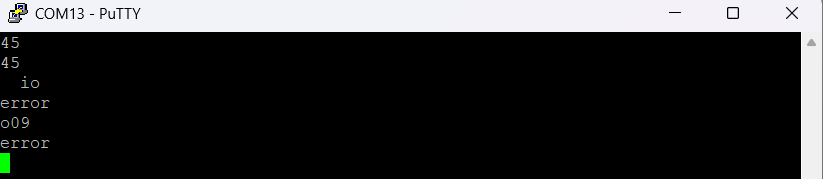
\includegraphics[width=\textwidth]{Resultados/salida_putty.png}
    \caption{Evidencia en PuTTY: eco de un numero y respuesta de \texttt{Error/error} para caracteres no numericos, ambos terminados en \texttt{CR+LF}.}
    \label{fig:putty-resultados}
\end{figure}


\end{document}
